


In this paper we have presented Sliceplorer, a visualization method for
multi-dimensional functions based on one-dimensional slices. We defined a task
taxonomy specific to multi-dimensional continuous functions and found that,
while some state of the art techniques are very good at  addressing specific
tasks, our method supports a wide variety of tasks. Consequently, our technique
may be a good first pass when visualizing multi-dimensional continuous functions. 
It is easy to implement, easy to understand, and addresses a greater variety
of tasks than any other technique. 

\begin{figure}
  \centering
  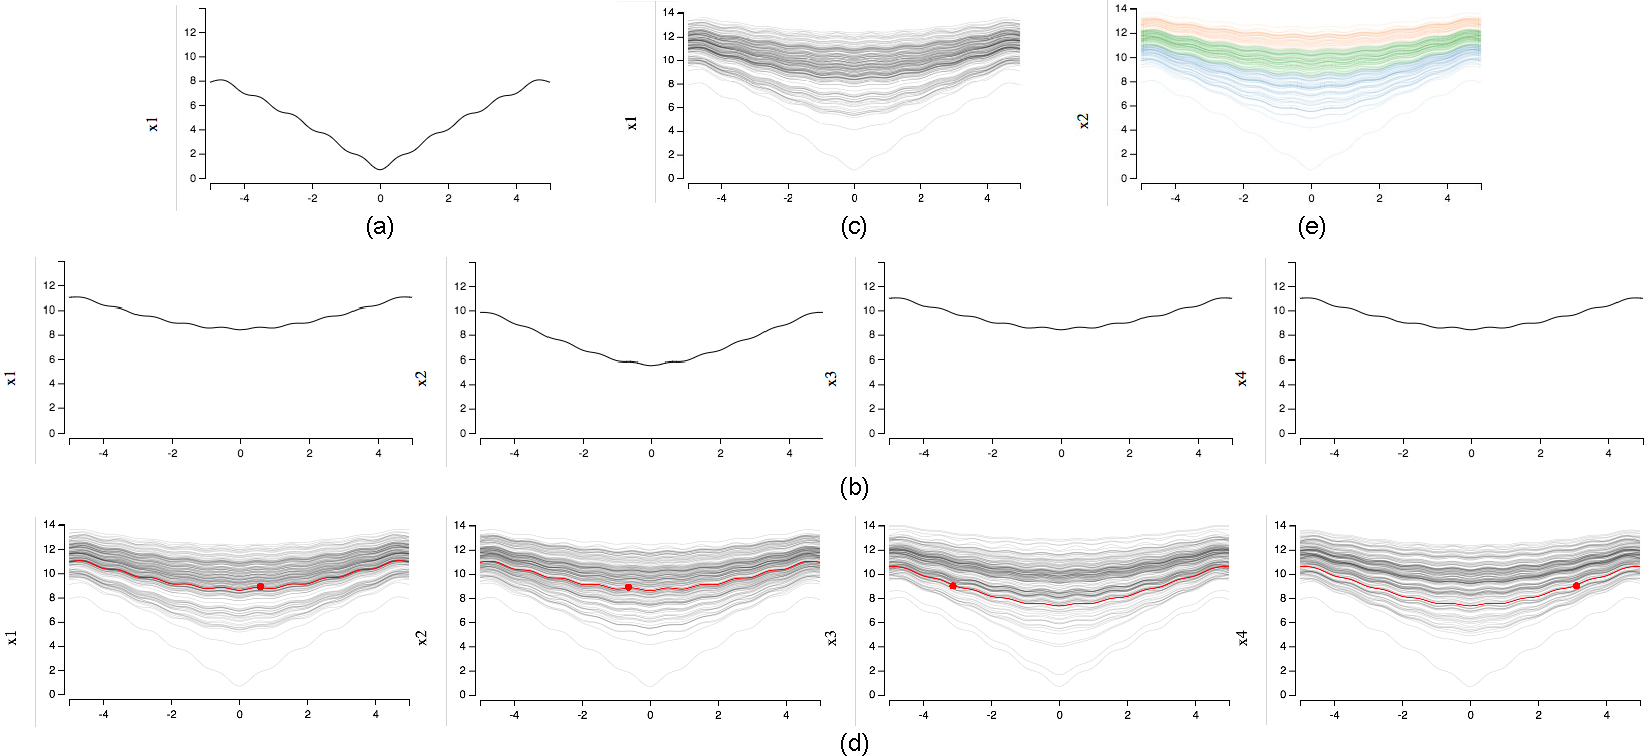
\includegraphics[width=0.9\textwidth]{sliceplorer_overview.pdf}
  \caption[The evolution of Sliceplorer.]{%
    The evolution of Sliceplorer. I adapt the commonly known technique of
    1D function plots (a) to
    multiple dimensions by taking a small multiples approach and repeating each
    plot for each dimension (b). I address the
    focus point selection problem by sampling over the parameter space and then
    projecting the slices in the corresponding plot
    (c). The user can mouse over a particular
    slice in one plot and the corresponding slices are highlighted in the other
    dimension plots (d). This allows one to
    see the corresponding function behaviors in the other dimensions.  Finally,
    one can cluster the function slices (e), to
    show groups of similar behavior in the manifold.
  }
  \label{fig:walkthrough}
\end{figure}


The visual analysis of multi-dimensional scalar functions is a fundamental aspect in many areas, from computational sciences (based on computer simulations) to data sciences (based on machine learning techniques) and general optimization algorithms. 
Neural networks, for instance, have shown to produce very good results that come in the form of highly non-linear response manifolds.
While understanding these manifolds would greatly help to verify
the resulting models, there
is currently no established way to inspect these multi-dimensional manifolds. 
In case of an optimization algorithm, a good visualization of response manifolds could, for instance, help to see where possible
``holes'' (local extrema) are that the algorithm may get trapped in and fail to find the
global optimum. By visually examining the functions that we are trying to
optimize, one can develop new insights on how to improve the optimization
algorithm. Our work is based on the assumption that visual analyses of these functions will help to increase
understanding of what they are doing, 
as argued by Gleicher~\cite{gleicher:2016}.

To examine these functions visually we must reduce them to be
displayed on a 2D screen. 
Currently, the two major approaches used to visualize these spaces are either
two-dimensional slices, a technique known as HyperSlice~\cite{Wijk:1993} or dimension transformation techniques. This includes dimensionality
reduction and topological methods~\cite{Correa:2011,Carr:2003a}.  HyperSlice
shows two-dimensional slices (using either a heatmap or contour view)
of the function directly around a particular focus point. It clearly shows the
behavior of the function with respect to the parameters. However, one can only
view one focus point at a time and 
the approach does not scale well to many dimensions.
With each additional dimension one must substantially 
shrink the subplots so less detail can be seen just like in scatterplot matrices. Topological and dimensionality
reduction techniques take the opposite approach. They morph the space to
produce a 2D global view. However, the morphing process is rather
complex and it is unclear what the resulting layout means. This reduces
comprehension. Ideally we would like to somehow combine the global view with
local detail.

In this paper, we explore the idea of 1D slices to fill this gap. We focus on 
multi-dimensional continuous scalar functions which we define as functions that take two or more
scalar parameters as input and produce a single scalar as output.
Towards illustrating the benefits, we propose a concrete technique using projections of 1D slices, which we call Sliceplorer (\autoref{fig:walkthrough}). 
1D slices are traditional function line plots familiar to anyone with
basic mathematics knowledge: one dimensional curves with respect to
changes in a single parameter. 
Like HyperSlice, we show a separate subplot
for each input dimension. For 1D slices, the number of
subplots scales linearly with the number of dimensions, not quadratically as with 2D slices. We address the issue of having to choose a focus
point by sampling focus points and then showing all slices as a
projection. Therefore, our 1D approach can be seen as a hybrid method of slicing
and projection techniques. 

In order to evaluate any new technique, we need to
consider what data characteristics and tasks each method is good for. As of yet, there has not been a comprehensive
listing of the tasks a user would want to perform when looking at
multi-dimensional continuous functions. To this
end, we begin development of this task summary by extending the task classification of Amar, Eagan, and Stasko~\cite{Amar:2005}. We use this classification to evaluate our 1D approach and compare it to 2D slices and different topological approaches. This comparison allows us to characterize what technique is best for which tasks and reveals that 1D slices is the most flexible of the current approaches. That is, it supports the broadest range of different tasks.

We also provide three usage scenarios comparing our technique with other state of the art techniques. These scenarios illustrate that 1D
slices can reveal structure in the functions that could not
have been seen before. For example, we discuss how one can use our
method to compare the \emph{global} prediction manifold of a neural
network algorithm against a support vector machine to guide and better understand the architecture of a neural network. This is currently an open research question in the machine learning community.

